%%%%%%%%%%%%%%%%%%%%%%%%%%%%%%%%%%%%%%%%%%%%%%%%%%%%%%%%%%%%%%%%
%%%%%%%%%%%%%%%%%%%%%%%%%%%%%%%%%%%%%%%%%%%%%%%%%%%%%%%%%%%%%%%%
%%%%
%%%% This text file is part of the source of 
%%%% `Introduction to High-Performance Scientific Computing'
%%%% by Victor Eijkhout, copyright 2012-6
%%%%
%%%% This book is distributed under a Creative Commons Attribution 3.0
%%%% Unported (CC BY 3.0) license and made possible by funding from
%%%% The Saylor Foundation \url{http://www.saylor.org}.
%%%%
%%%%
%%%%%%%%%%%%%%%%%%%%%%%%%%%%%%%%%%%%%%%%%%%%%%%%%%%%%%%%%%%%%%%%
%%%%%%%%%%%%%%%%%%%%%%%%%%%%%%%%%%%%%%%%%%%%%%%%%%%%%%%%%%%%%%%%

\emph{Source code control}\index{source code control} systems, also
called \emph{revision control}\index{revision control
  systems|see{source code control}}  or
\emph{version control}\index{version control systems|see{source code control}}
systems, are
a way of storing software, where not only the current version is
stored, but also all previous versions. 
This is done by maintaining a \indexterm{repository} for all versions,
while one or more users work on a `checked out' copy of the latest
version. Those of the users that are developers can then commit their
changes to the repository. Other users then update their local copy.
The repository typically resides on a remote machine that is reliably
backup up.

There are various reasons for keeping your source in a repository.
\begin{itemize}
\item If you work in a team, it is the best way to synchronize your
  work with your colleagues. It is also a way to document what changes
  were made, by whom, and why.
\item It will allow you to roll back a defective code to a version
  that worked.
\item It allows you to have branches, for instance for customizations
  that need to be kept out of the main development line. If you are
  working in a team, a branch is a way to develop a major feature, stay up
  to date with changes your colleagues make, and only add your feature
  to the main development when it is sufficiently tested.
\item If you work alone, it is a way to synchronize between more than
  one machine. (You could even imagine traveling without all your
  files, and installing them from the repository onto a borrowed
  machine as the need arises.)
\item Having a source code repository is one way to backup your work.
\end{itemize}

There are various source code control systems; in this tutorial you
can learn the basics of \indexterm{Subversion} (also called
\emph{svn}), which is probably the most popular of the traditional
source code control systems, and Mercurial (or~\n{hg}), which is an
example of the new generation of \indextermsub{distributed}{source
code control} systems.

\Level 0 {Workflow in source code control systems}

Source code control systems are built around the notion
of \indexterm{repository}: a central store of the files of a project,
together with their whole history. Thus, a repository allows you to
share files with multiple people, but also to roll back changes, apply
patches to old version, et cetera.

The basic actions on a repository are:
\begin{itemize}
\item Creating the repository; this requires you to have space and
  write permissions on some server. Maybe your sysadmin has to do it
  for you.
\item Checking out the repository, that is, making a local copy of its
  contents in your own space.
\item\label{it:commit} Adding your changes to the repository, and
\item Updating your local copy with someone else's changes.
\end{itemize}
Adding your own changes is not always possible: there are many projects
where the developer allows you to check out the repository, but not to
incorporate changes. Such a repository is said to be read-only.

Figure~\ref{fig:svn} illustrates these actions for the Subversion system.
\begin{figure}[ht]
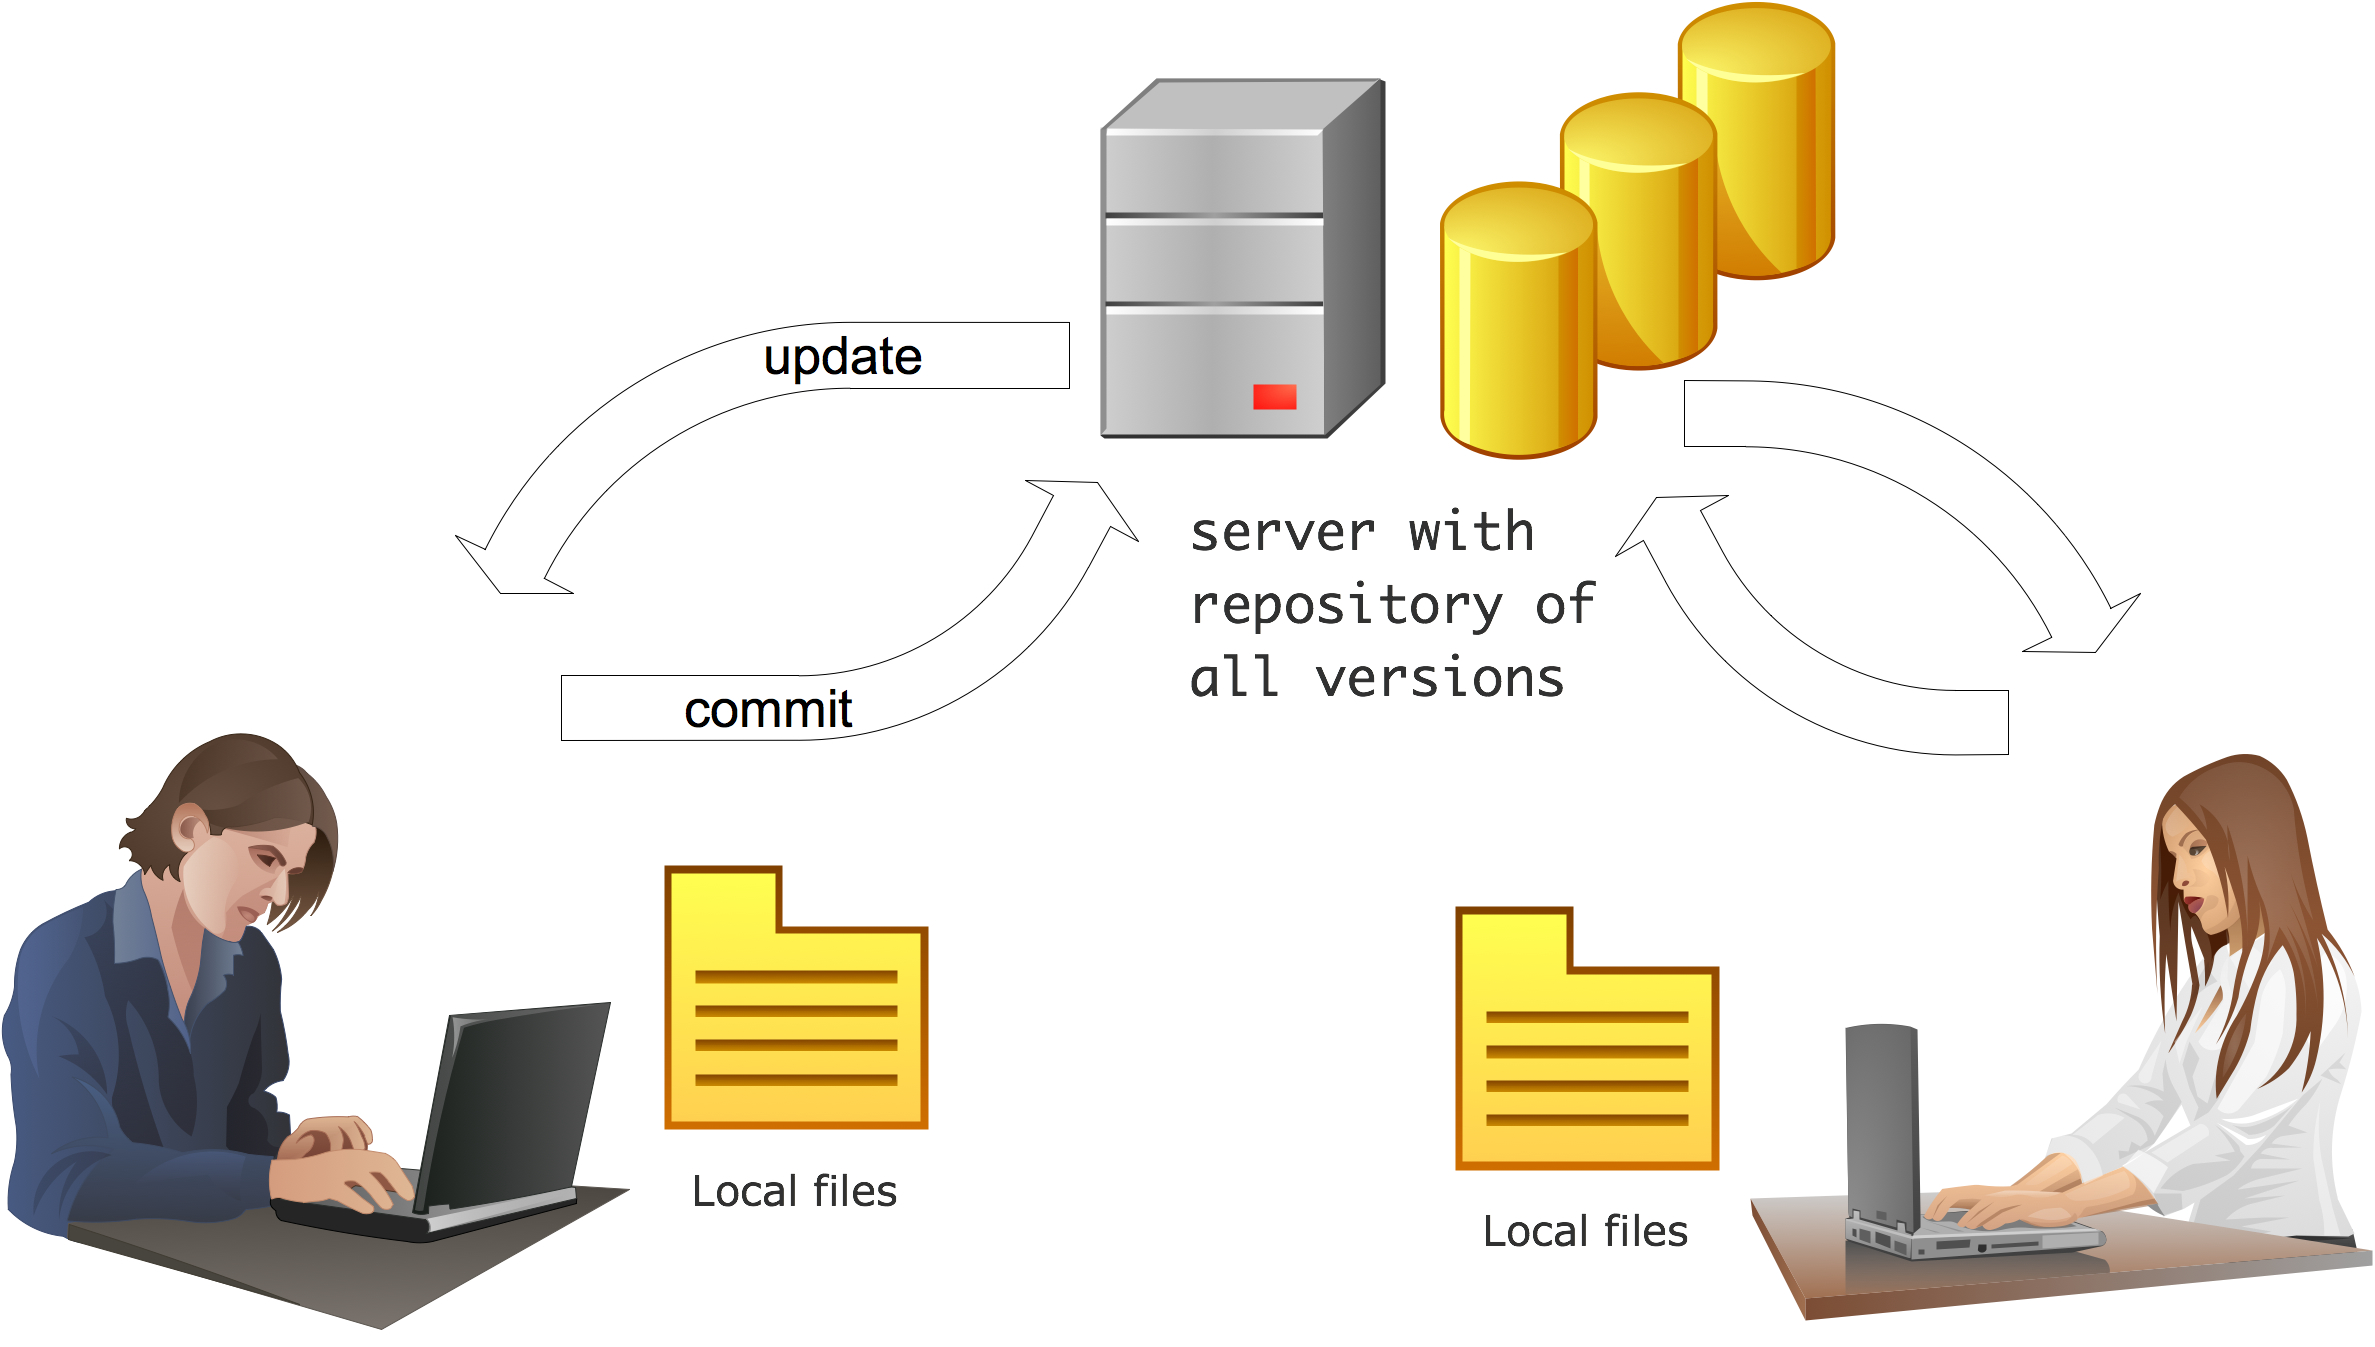
\includegraphics[scale=.17]{graphics/repo-flow-svn}
\caption{Workflow in traditional source code control systems such as Subversion}
\label{fig:svn}
\end{figure}
Users who have checked out the repository can edit files, and check in
the new versions with the \n{commit} command; to get the changes
committed by other users you use \n{update}.

One of the uses of committing is that you can roll your code back to
an earlier version if you realize you made a mistake or introduced a
bug. It also allows you to easily see the difference between different
code version. However, committing many small changes may be confusing
to other developers, for instance if they come to rely on something
you introduce which you later remove again. For this reason,
\indextermsub{distributed}{source code control} systems use two levels
of repositories.

There is still a top level that is authoritative, but
now there is a lower level, typically of local copies, where you can
commit your changes and accumulate them until you finally add them to
the central repository.
\begin{figure}[ht]
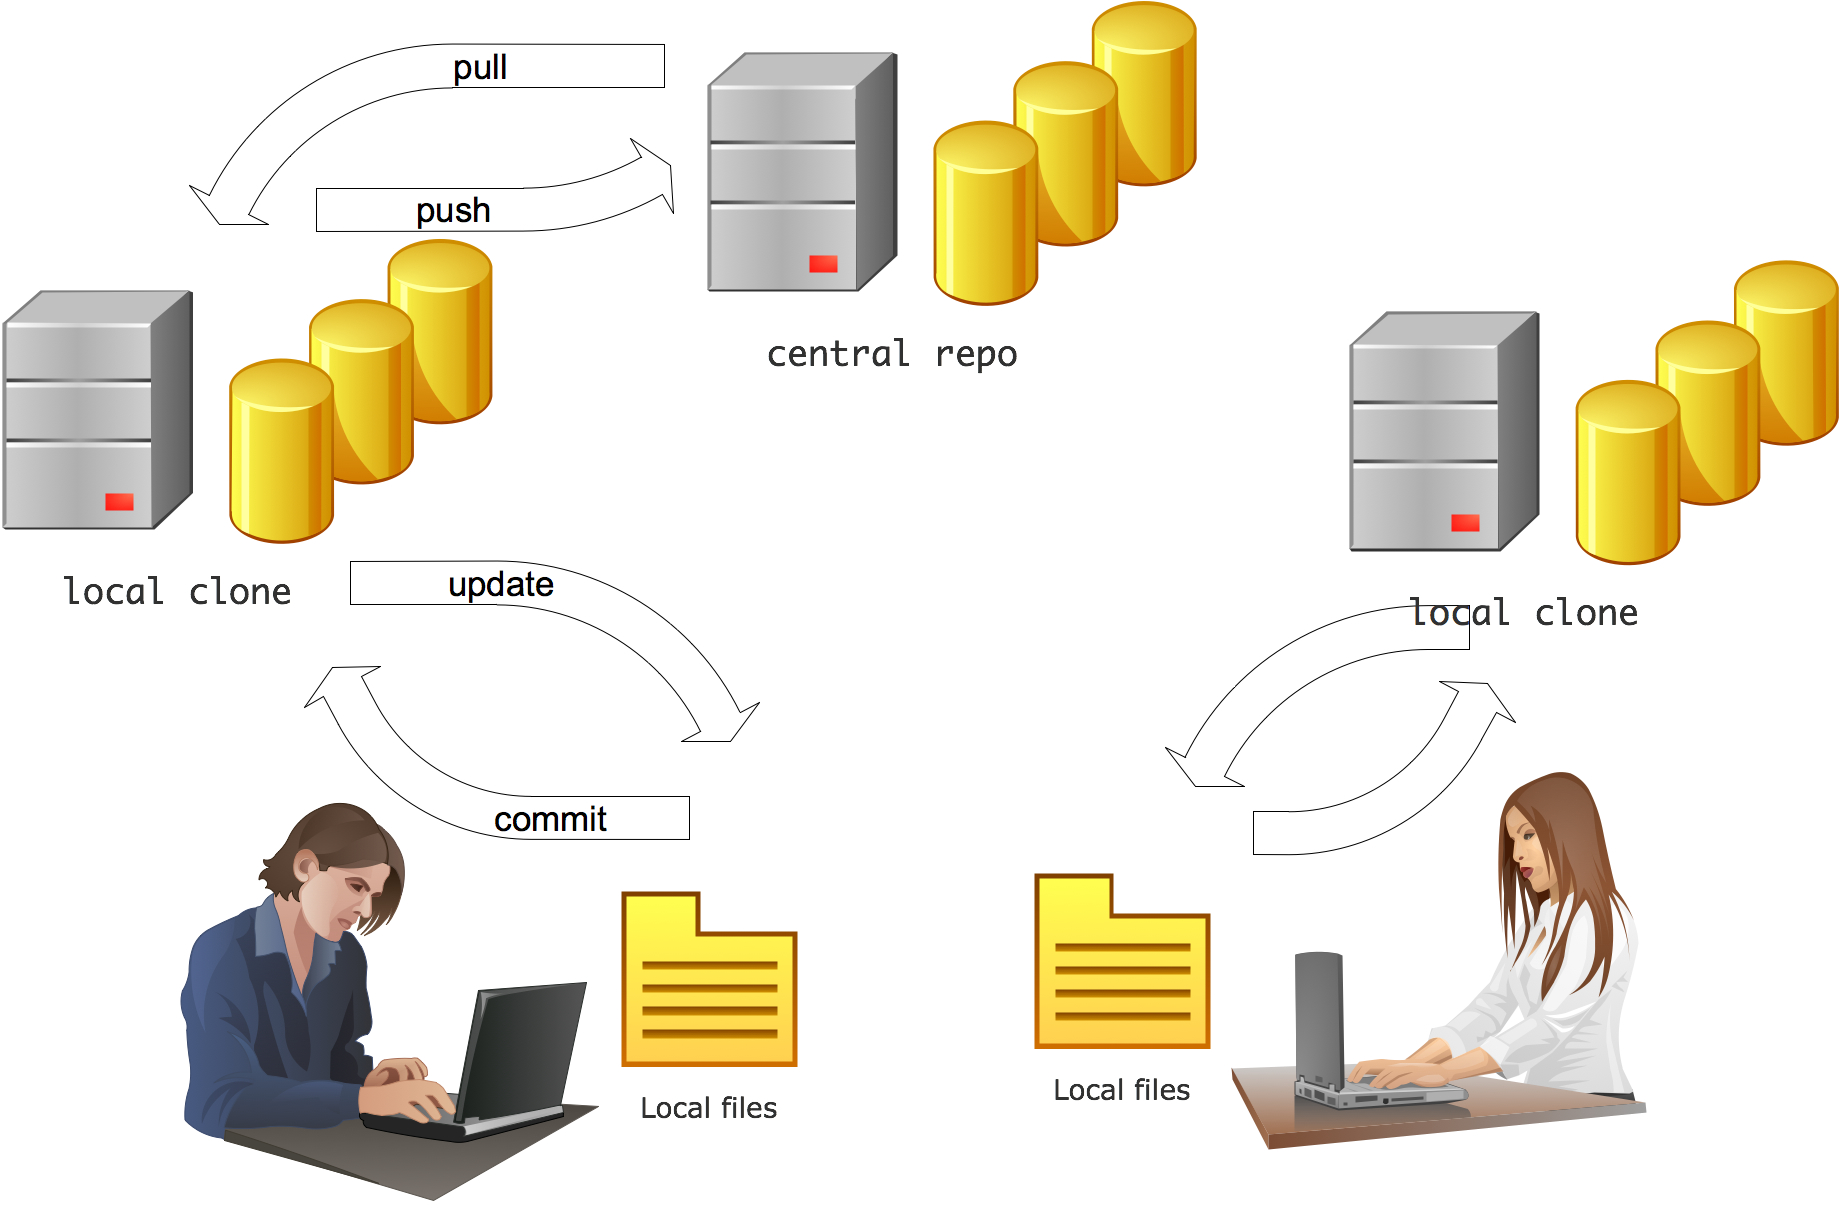
\includegraphics[scale=.19]{graphics/repo-flow-hg}
\caption{Workflow in distributed source code control systems such as Mercurial}
\label{fig:hg}
\end{figure}
This also makes it easier to contribute to a read-only repository:
you make your local changes, and when you are finished you tell the 
developer to inspect your changes and pull them into the top level 
repository. This structure is illustrated in figure~\ref{fig:hg}.

%\input tutorials/subversion
\input tutorials/mercurial
